\section{The simulation of muons in the SiD detector}
\label{Detector}

In the first step of simulating the muons in the SiD detector, event displays were made with WIRED4.
The xy- and zy-views of these event displays can be seen for both shielding scenarios in Figure~\ref{fig:WIRED4}.
When comparing the figures, one can notice several things about the number and the spatial distribution of the hits in the detector.
First of all, without the magnetized wall as a last shielding mechanism about 6 times more muons find their way into the interaction region.
In these plots as in all following, the shown distributions are from muons from one ILC bunch train, since the SiD sensor buffers will be read out after every train only.\\
Second, the muons travel through the detector horizontally which could be taken advantage of for the alignment of the subdetectors.
The spatial distributions of the muons in both scenarios are shifted towards the top and the left.
The reason for the top-bottom and left-right asymmetry is the shielding ability of the tunnel walls and floor.
Since the detector hall is set into the floor, and the BDS system is curved, only the muons being emitted in such a way that they get through the tunnel opening to the detector hall hit the detector.
Finally, the most significant difference between the two scenarios is the broad spatial distribution for the scenario with the wall in comparison to the distinct distribution in the '5 Spoilers' scenario.
The magnetized wall deflects the muons and also stops the low energy ones, so that the muon rate is reduced and the muons are additionally distributed over the whole detector area.
Figure~\ref{fig:muon_energy} shows the muon energy distributions for both shielding scenarios.

\begin{figure}
    \centering
    \begin{subfigure}[b]{0.49\textwidth}
    \begin{center}
        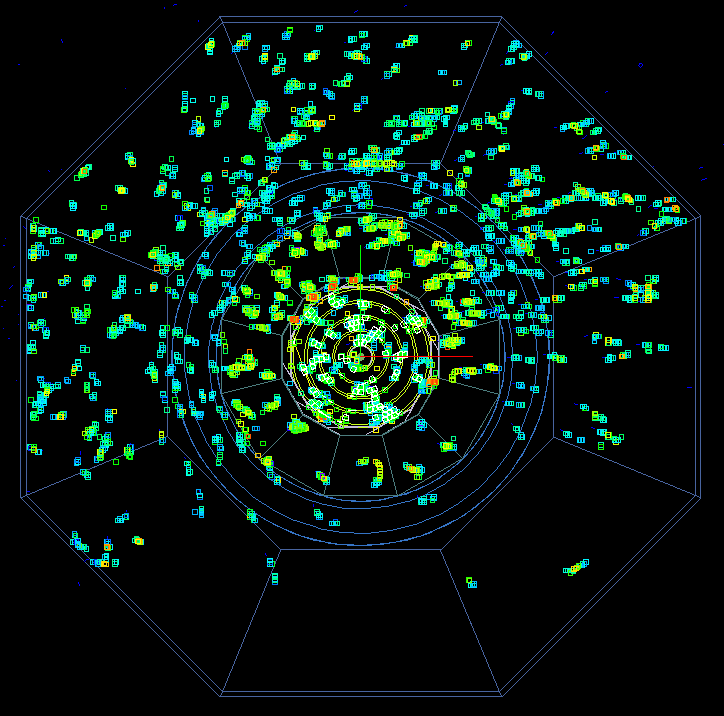
\includegraphics[height=0.3\textheight]{figures/muons_positron_5spoilers_wall_515_xyview_croped.png}
        \caption{xy-view, '5 Spoilers + Wall'}
	\label{fig:xy_5SpoilersWall}
    \end{center}
    \end{subfigure}
    \begin{subfigure}[b]{0.49\textwidth}
    \begin{center}
        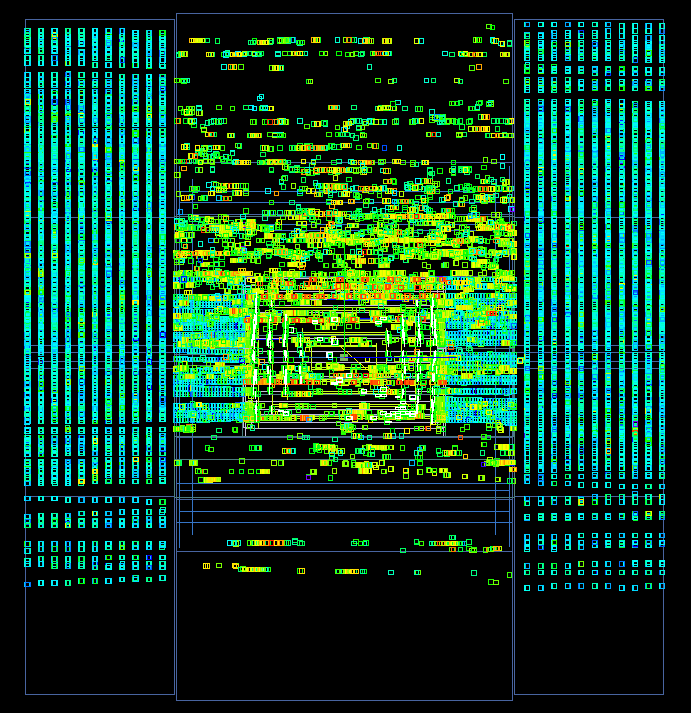
\includegraphics[height=0.3\textheight]{figures/muons_positron_5spoilers_wall_515_zyview_croped.png}
        \caption{zy-view, '5 Spoilers + Wall'}
        \label{fig:zy_5SpoilersWall}
    \end{center}
    \end{subfigure}\\
    \begin{subfigure}[b]{0.49\textwidth}
    \begin{center}
        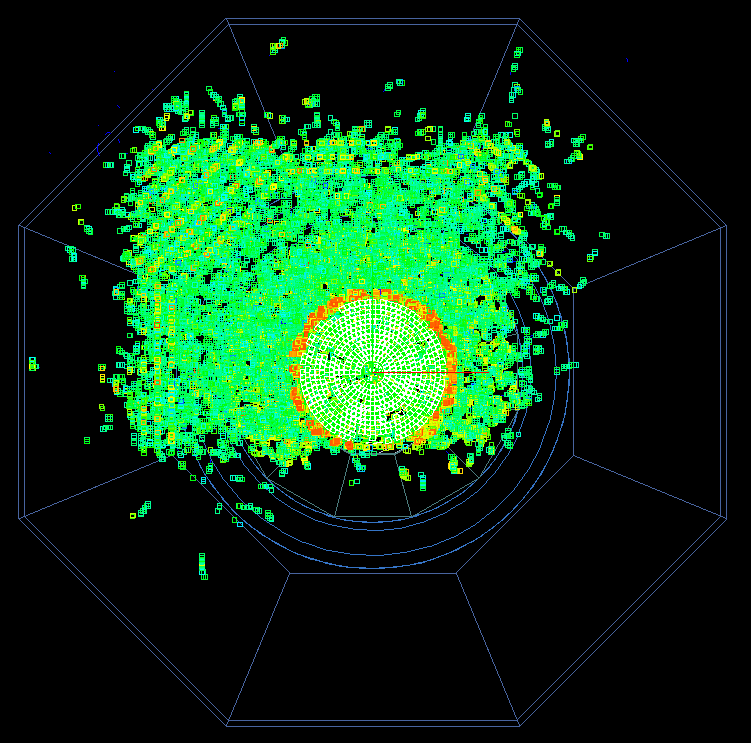
\includegraphics[height=0.3\textheight]{figures/muons_positron_5spoilers_2961_xyview_croped.png}
        \caption{xy-view, '5 Spoilers'}
	\label{fig:xy_5Spoilers}
    \end{center}
    \end{subfigure}
    \begin{subfigure}[b]{0.49\textwidth}
    \begin{center}
        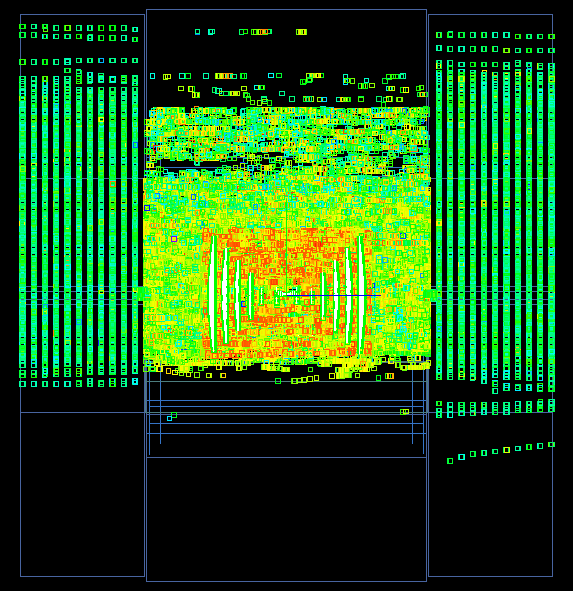
\includegraphics[height=0.3\textheight]{figures/muons_positron_5spoilers_2961_zyview_croped.png}
        \caption{zy-view, '5 Spoilers'}
        \label{fig:zy_5Spoilers}
    \end{center}
    \end{subfigure}
    \caption[Event displays of muons in SiD]{
    Event displays in the xy- and zy-view of the muons from the '5 Spoilers + Wall' and '5 Spoilers' scenario in the SiD detector.
    Figures a) and b) show hits from 515 muons with the magnetized wall, and c) and d) show hits from 2961 muons without the wall.
    The number of muons corresponds to the number of muons accumulated over one ILC bunch train (1312 bunch crossings), but in both cases the muons come from the positron line of the BDS only.
    Hence, one had to imagine roughly double the amount of hits in the SiD detector to get the full picture of all hits from muons from one bunch train.
    }
    \label{fig:WIRED4}
\end{figure}

\begin{figure}
    \centering
    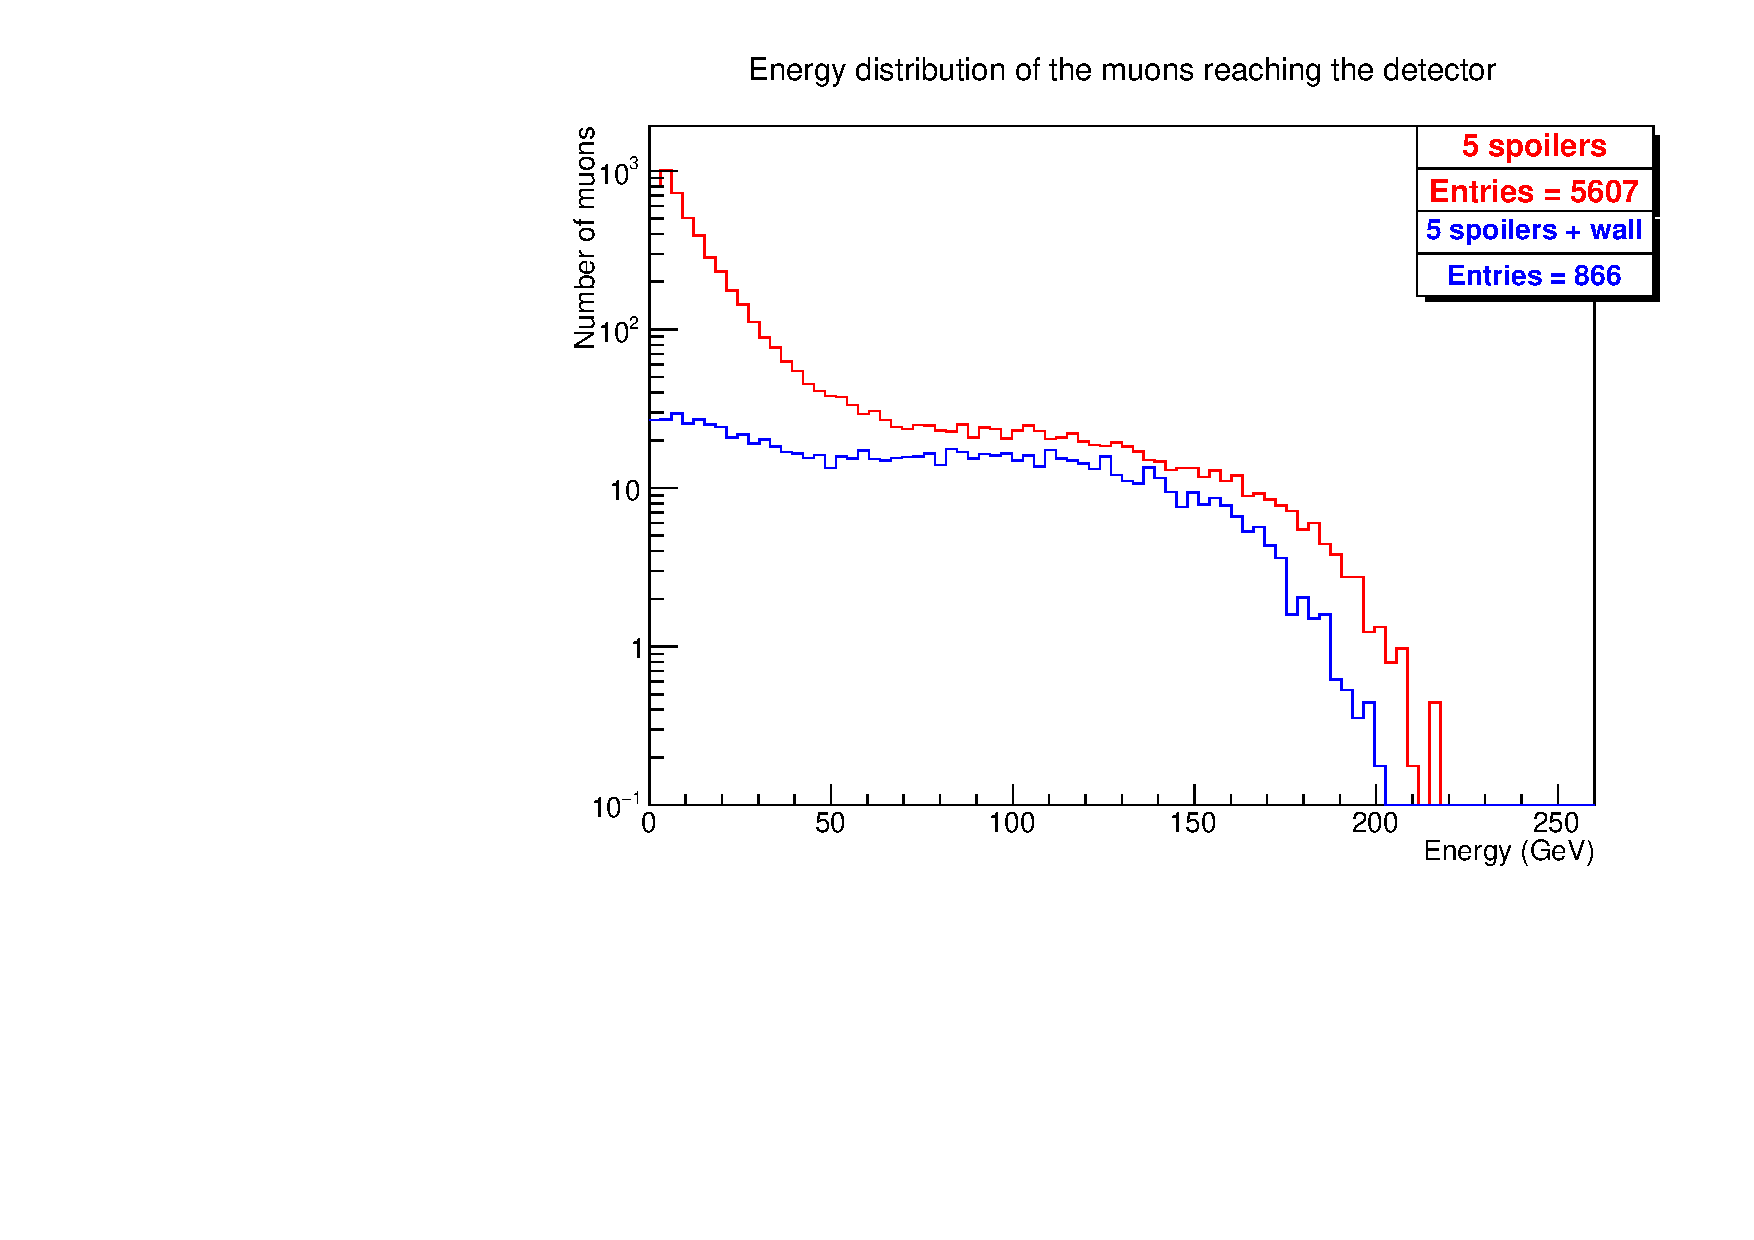
\includegraphics[width=0.7\textwidth]{figures/muon_energy.pdf}
    \caption[Energy distribution of muons from the two shielding scenarios]{
    The energy distributions of the muons from one ILC bunch train (1312 bunch crossings) for both scenarios, '5 Spoilers' (red) and '5 Spoilers + Wall' (blue), show that magnetized wall deflects and stops the low energy muons.
    The peak for low energies is therefore missing in the second scenario, and the whole distribution is shifted towards low energies.
    }
    \label{fig:muon_energy}
\end{figure}

The difference in the spatial distributions explains the different numbers of hits in the single subdetectors for the two scenarios.
With the muon endcaps having the largest effective detector area, the number of hits is the highest in this subdetector.

\begin{figure}
    \centering
    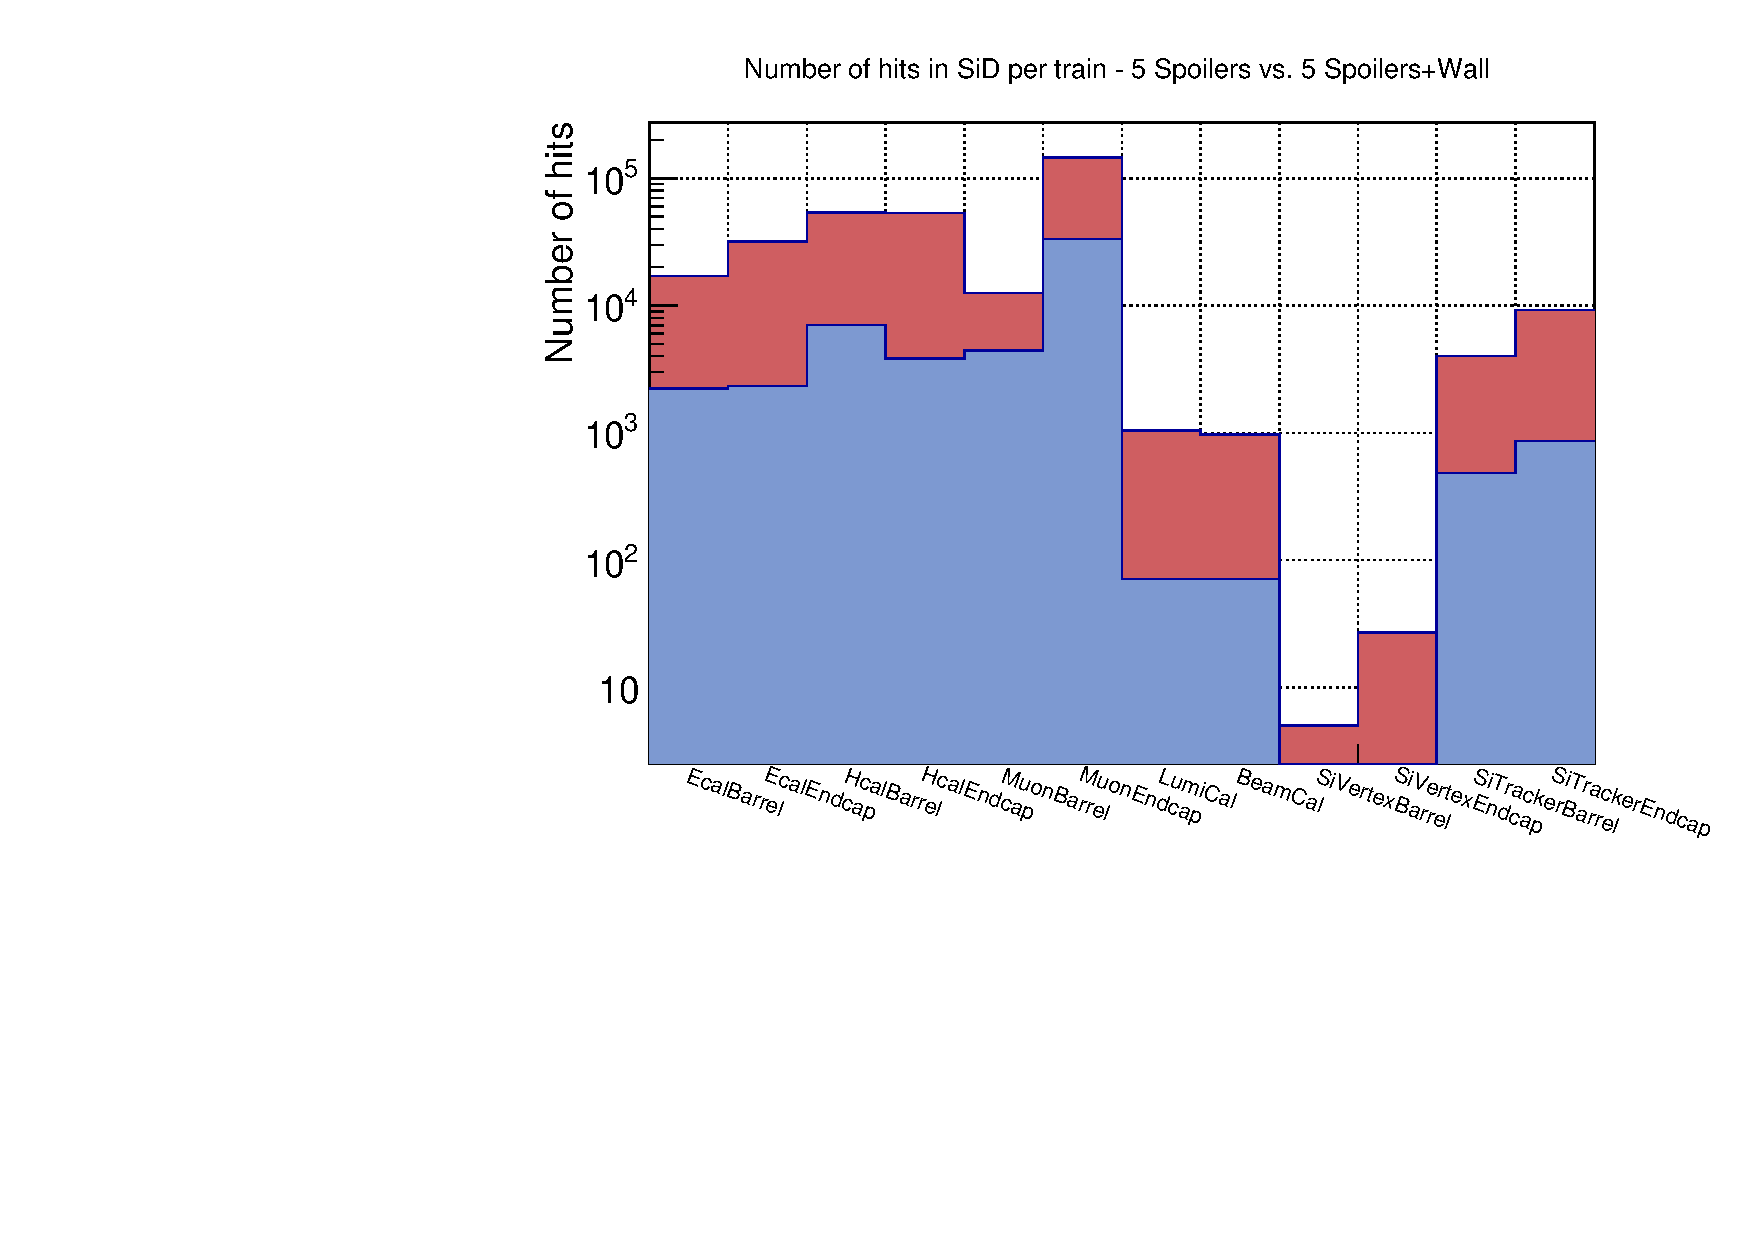
\includegraphics[width=\textwidth]{figures/Hits_in_SiD_subdetectors_MuonSpoilerStudy.pdf}
    \caption[Hit number distribution in the SiD subdetectors]{
    The hit number distributions of the muon hits in the SiD subdetectors from one ILC bunch train (1312 bunch crossings).
    The two scenarios are colored in red ('5 Spoilers') and blue ('5 Spoilers + Wall') as before.
    The number of hits is proportional to the effective detector area.
    Since the muons travel horizontally through the detector from one side to the other, the detector with the biggest effective area perpendicular to the muon incidence has the highest number of hits.
    }
    \label{fig:hit_distribution}
\end{figure}

Figure~\ref{fig:Occupancy_DeadCells} shows the occupancy plots and the number of dead cells resulting from the occupancy for both scenarios, and for two different subdetectors: the tracker endcaps and the ECAL endcaps.
The occupancy in the tracker endcaps (Figure~\ref{fig:SiTracker_Occupancy}) is very low for both scenarios.
Only 10\textsuperscript{-9} - 10\textsuperscript{-7} of all hits get four hits.
The resulting number of dead cells in the tracker endcaps (Figure~\ref{fig:SiTracker_DeadCells}) shows that for a buffer depth of 4 only 10\textsuperscript{-8} of all cells get four or more hits and therefore reach the buffer limit in the '5 Spoilers + Wall'.
The '5 Spoilers' case would do only one order of magnitude better.\\
More interesting are the plots for the ECAL endcaps in Figures~\ref{fig:Ecal_Occupancy} and \ref{fig:Ecal_DeadCells}.
The occupancy is for both cases higher than for the tracker endcaps, which is simply due to the bigger effective detector area as explained before.
Despite that and the fact that the ’5 Spoilers + Wall’ case is better by an order of magnitude (when looking at a buffer depth of 4), the occupancy is still at a level of only about 10\textsuperscript{−6} - 10\textsuperscript{−5}.
The interesting fact is that the ’5 Spoilers’ case shows up to 27 hits per cell with a roughly constant occupancy for all buffer depths.
This leads to dead cell distributions which are vastly different.
For an assumed buffer depth of 4, the total number of dead cells is different by about two orders of magnitude when comparing the two shielding scenarios.
In the ’5 Spoilers’ case, 10\textsuperscript{−4} - 10\textsuperscript{−3} cells would have reached the buffer limit regardless of which buffer depth was chosen for the sensor design.
The cause of this distribution is the spatial distribution of the muons in the ’5 Spoilers’ case: there are many more muons hitting the detector, and additionally all concentrated on a small area of the detector.

\begin{figure}
    \centering
    \begin{subfigure}[b]{0.49\textwidth}
    \centering
        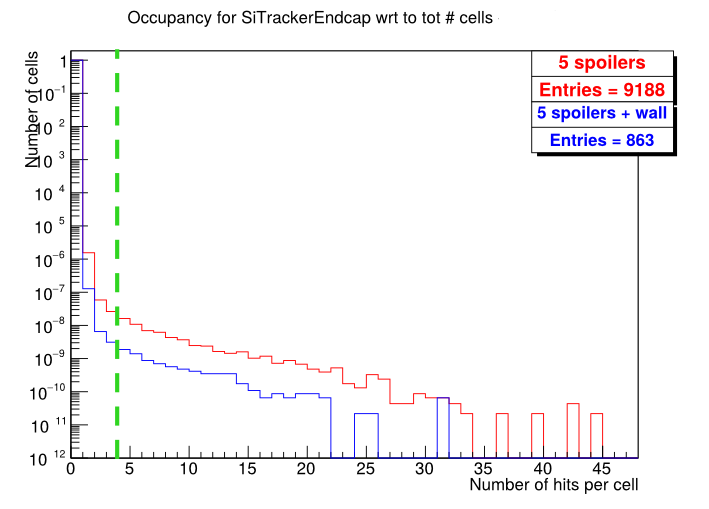
\includegraphics[height=0.27\textheight]{figures/SiTrackerEndcap_Occupancy.png}
        \caption{Tracker endcap occupancy}
	\label{fig:SiTracker_Occupancy}
    \end{subfigure}
    \begin{subfigure}[b]{0.49\textwidth}
    \centering
        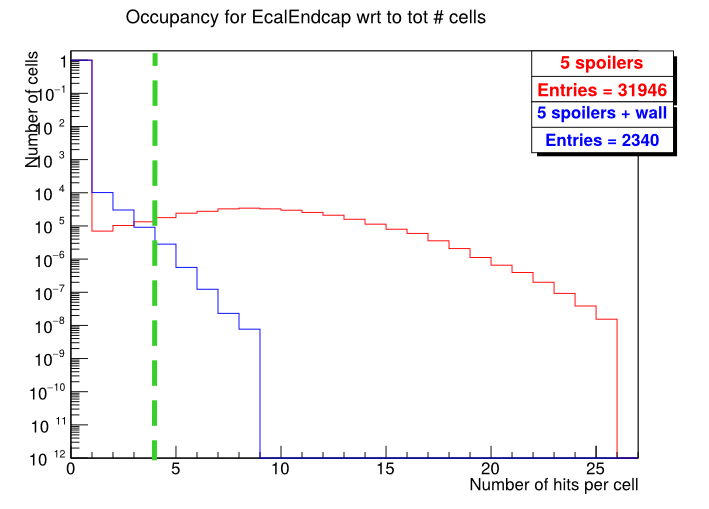
\includegraphics[height=0.27\textheight]{figures/EcalEndcap_Occupancy.png}
        \caption{ECAL endcap occupancy}
        \label{fig:Ecal_Occupancy}
    \end{subfigure}\\
    \begin{subfigure}[b]{0.49\textwidth}
    \centering
        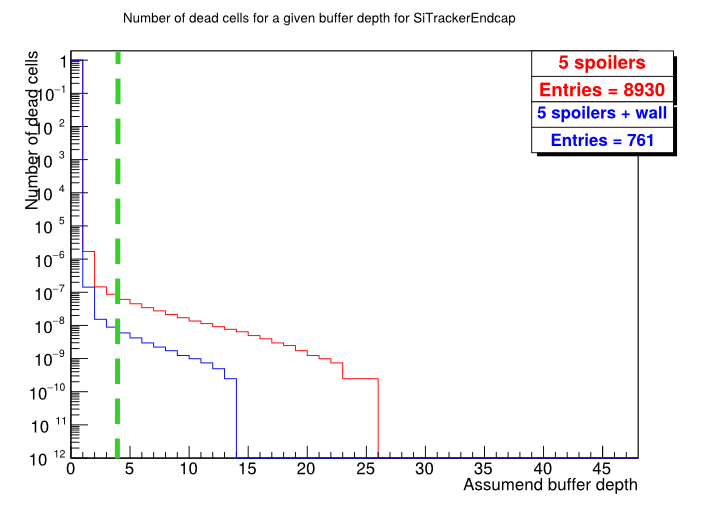
\includegraphics[height=0.27\textheight]{figures/SiTrackerEndcap_DeadCells.png}
        \caption{Dead cells in the tracker endcaps}
	\label{fig:SiTracker_DeadCells}
    \end{subfigure}
    \begin{subfigure}[b]{0.49\textwidth}
    \centering
        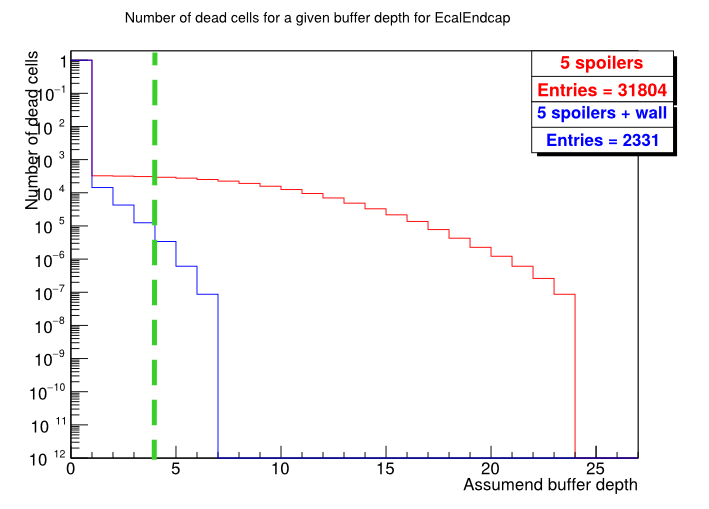
\includegraphics[height=0.27\textheight]{figures/EcalEndcap_DeadCells.png}
        \caption{Dead cells in the ECAL endcaps}
        \label{fig:Ecal_DeadCells}
    \end{subfigure}
    \caption[Muon occupancy in the tracker endcaps and ECAL endcaps]{
    Figures ~\ref{fig:SiTracker_Occupancy} and \ref{fig:Ecal_Occupancy} show for both shielding scenarios the muon occupancy in the tracker endcaps and the ECAL endcaps, i.e. the fraction of all cells that are hit a certain number of times.
    The plots are normalized by the total number of cells in this subdetector.\\
    Figures~\ref{fig:SiTracker_DeadCells} and \ref{fig:Ecal_DeadCells} show in comparison the number of dead cells which is the result of the occupancy and the buffer depth of the sensors.
    For a given buffer depth, all cells with hit numbers greater or equal than the buffer depth are 'dead', and therefore blind to all following hits.
    Therefore, in the hypothetical case of a buffer depth of 0, all cells are dead.\\
    In all plots, the green dashed line represents the buffer depth of the current sensor design.
    }
    \label{fig:Occupancy_DeadCells}
\end{figure}

Finally, also the timing of the muons with respect to the bunch crossing was studied.
All of the muons from the BDS are created up to \unit{0.5}{ns} after the bunch passing the material, as can be seen in Figure~\ref{fig:Creation_time}.
Although the muons are created instantaneously, it takes a long time for them to hit certain subdetectors, like the inner lying ECAL.
The muons have to travel through the outer subdetectors before they reach the ECAL endcaps, which takes about \unit{20}{ns}.
After roughly another \unit{20}{ns} the second endcap has been reached, so that hits in the ECAL endcaps can be registered several \unit{10}{ns} after the bunch crossing .
The muons also produce shower particles when passing through the whole detector material.
The low energy shower particles then hit the ECAL endcaps even later than the primary muons.

\begin{figure}
    \centering
    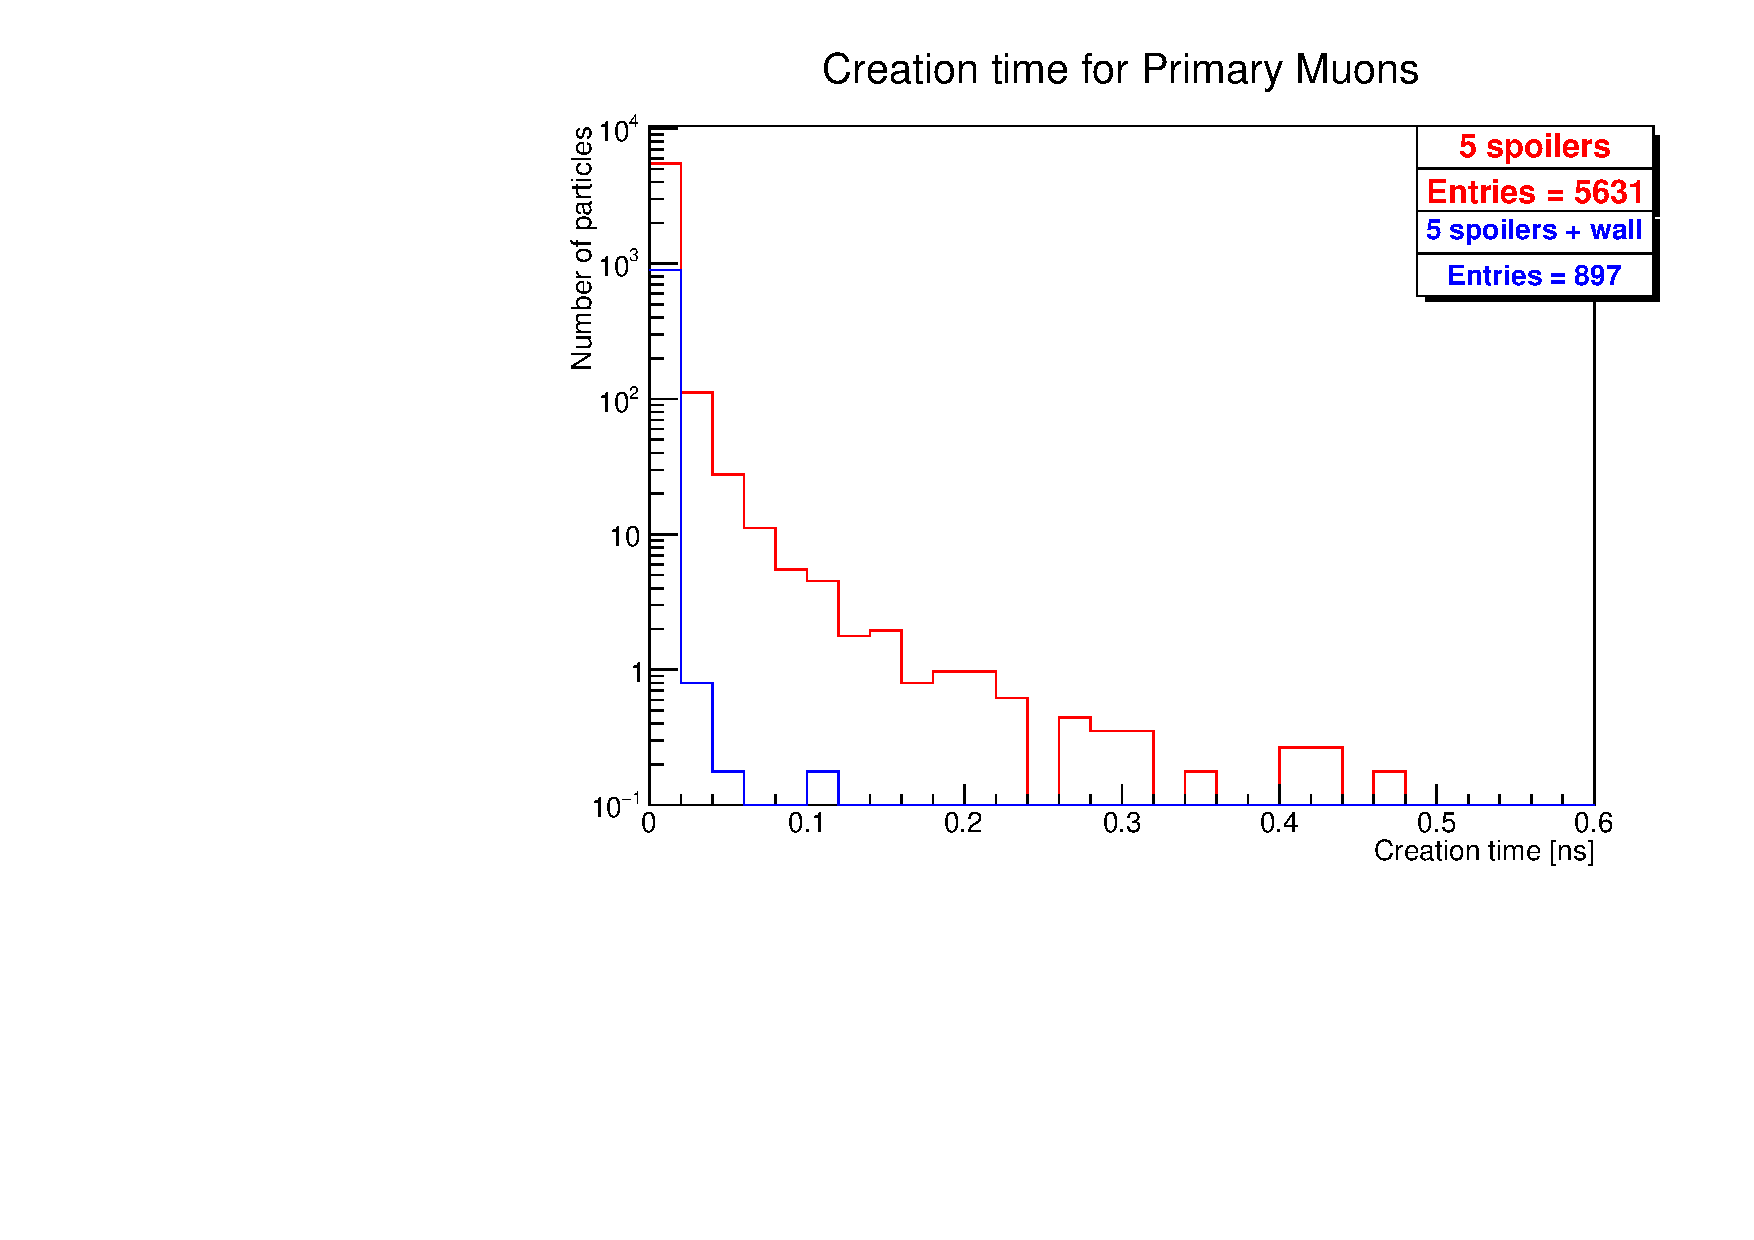
\includegraphics[width=0.7\textwidth]{figures/muon_creationtime.pdf}
    \caption[Creation time of the muons]{
    The creation time of the muons from the two shielding scenarios for a full bunch train.
    All of the muons from the BDS are created up to 0.5 ns after the bunch passing the material, whereas the lower energy muons, which have a broader creation time, do not reach the detector in the ’5 Spoilers + Wall’ case.
    }
    \label{fig:Creation_time}
\end{figure}
\begin{figure}
    \centering
    \begin{subfigure}[b]{0.49\textwidth}
    \centering
        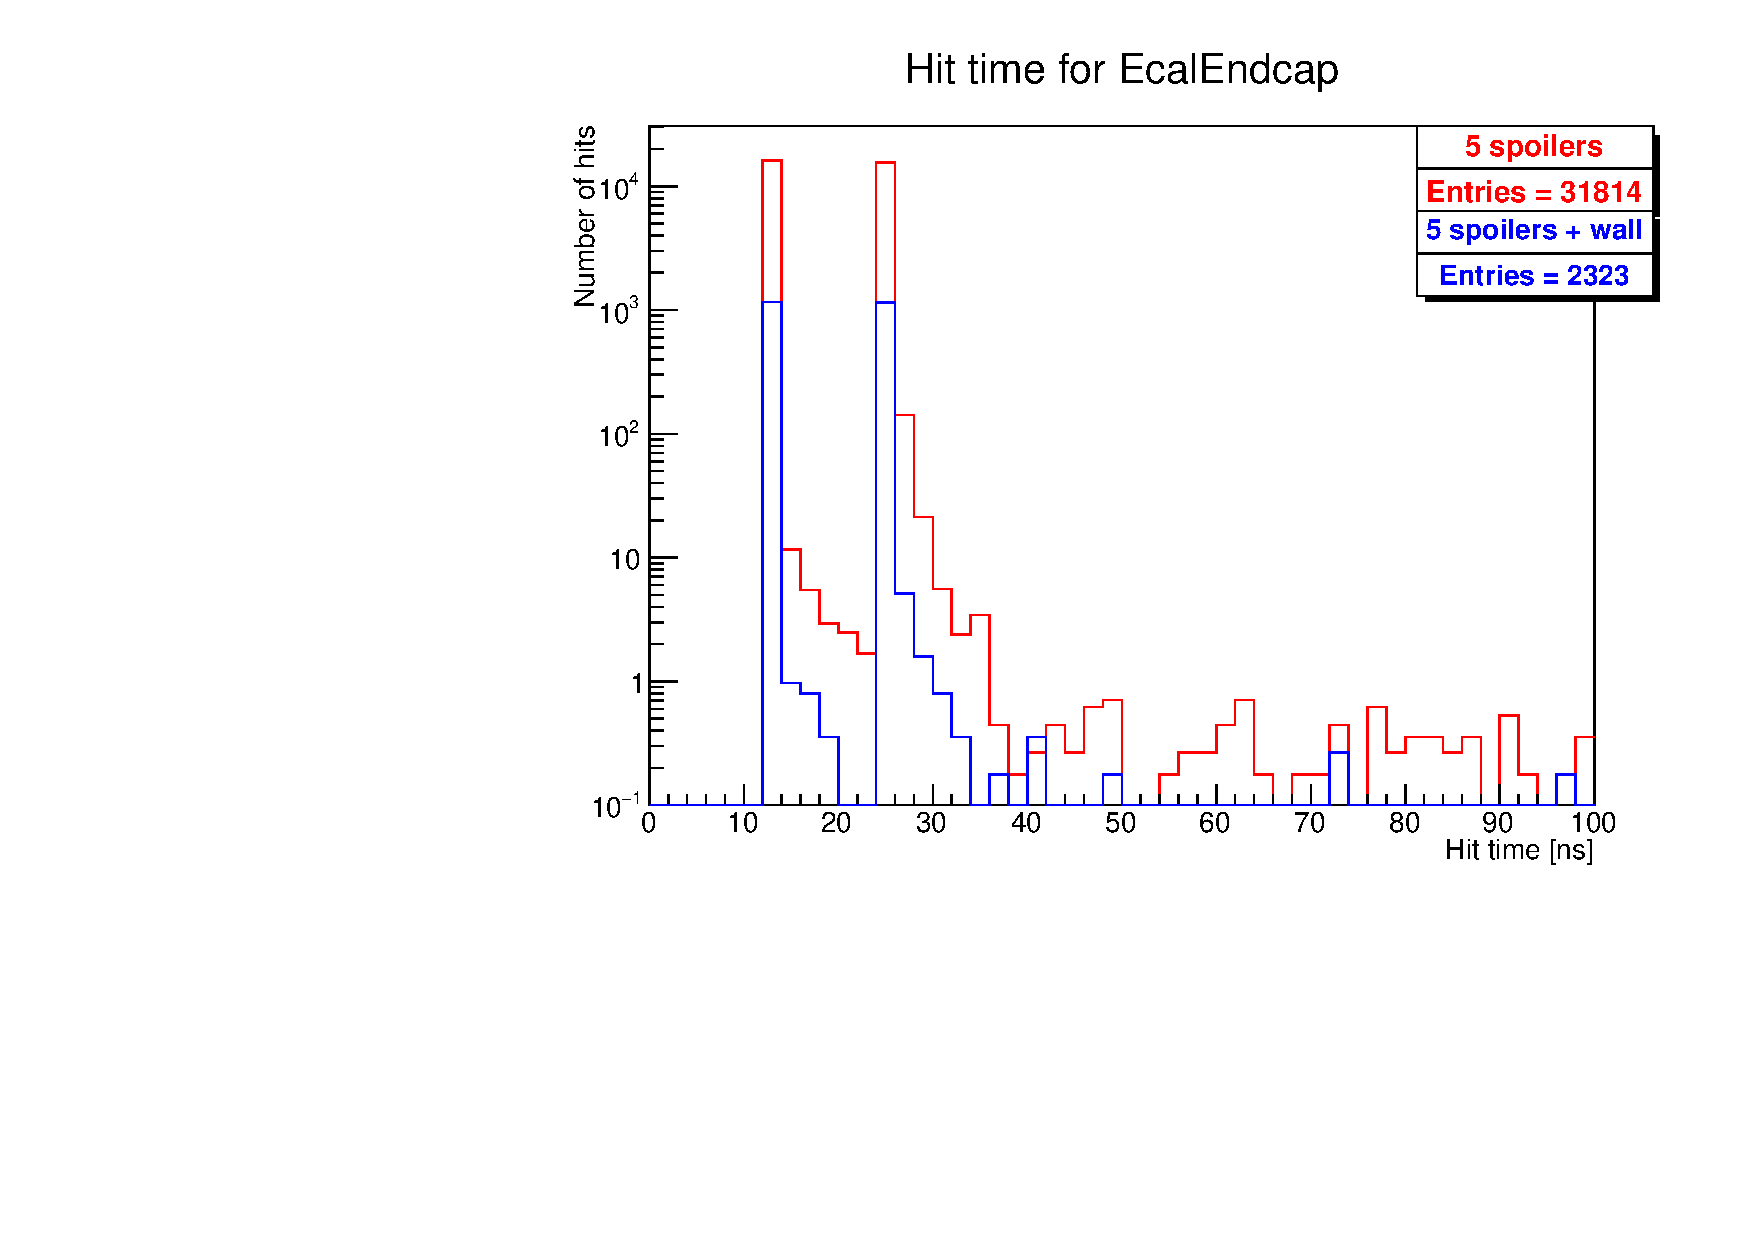
\includegraphics[height=0.26\textheight]{figures/muon_hittime_all_layers_EcalEndcap.pdf}
        \caption{Hit time of the primary muons}
	\label{fig:hittime_ECAL}
    \end{subfigure}
    \begin{subfigure}[b]{0.49\textwidth}
    \centering
        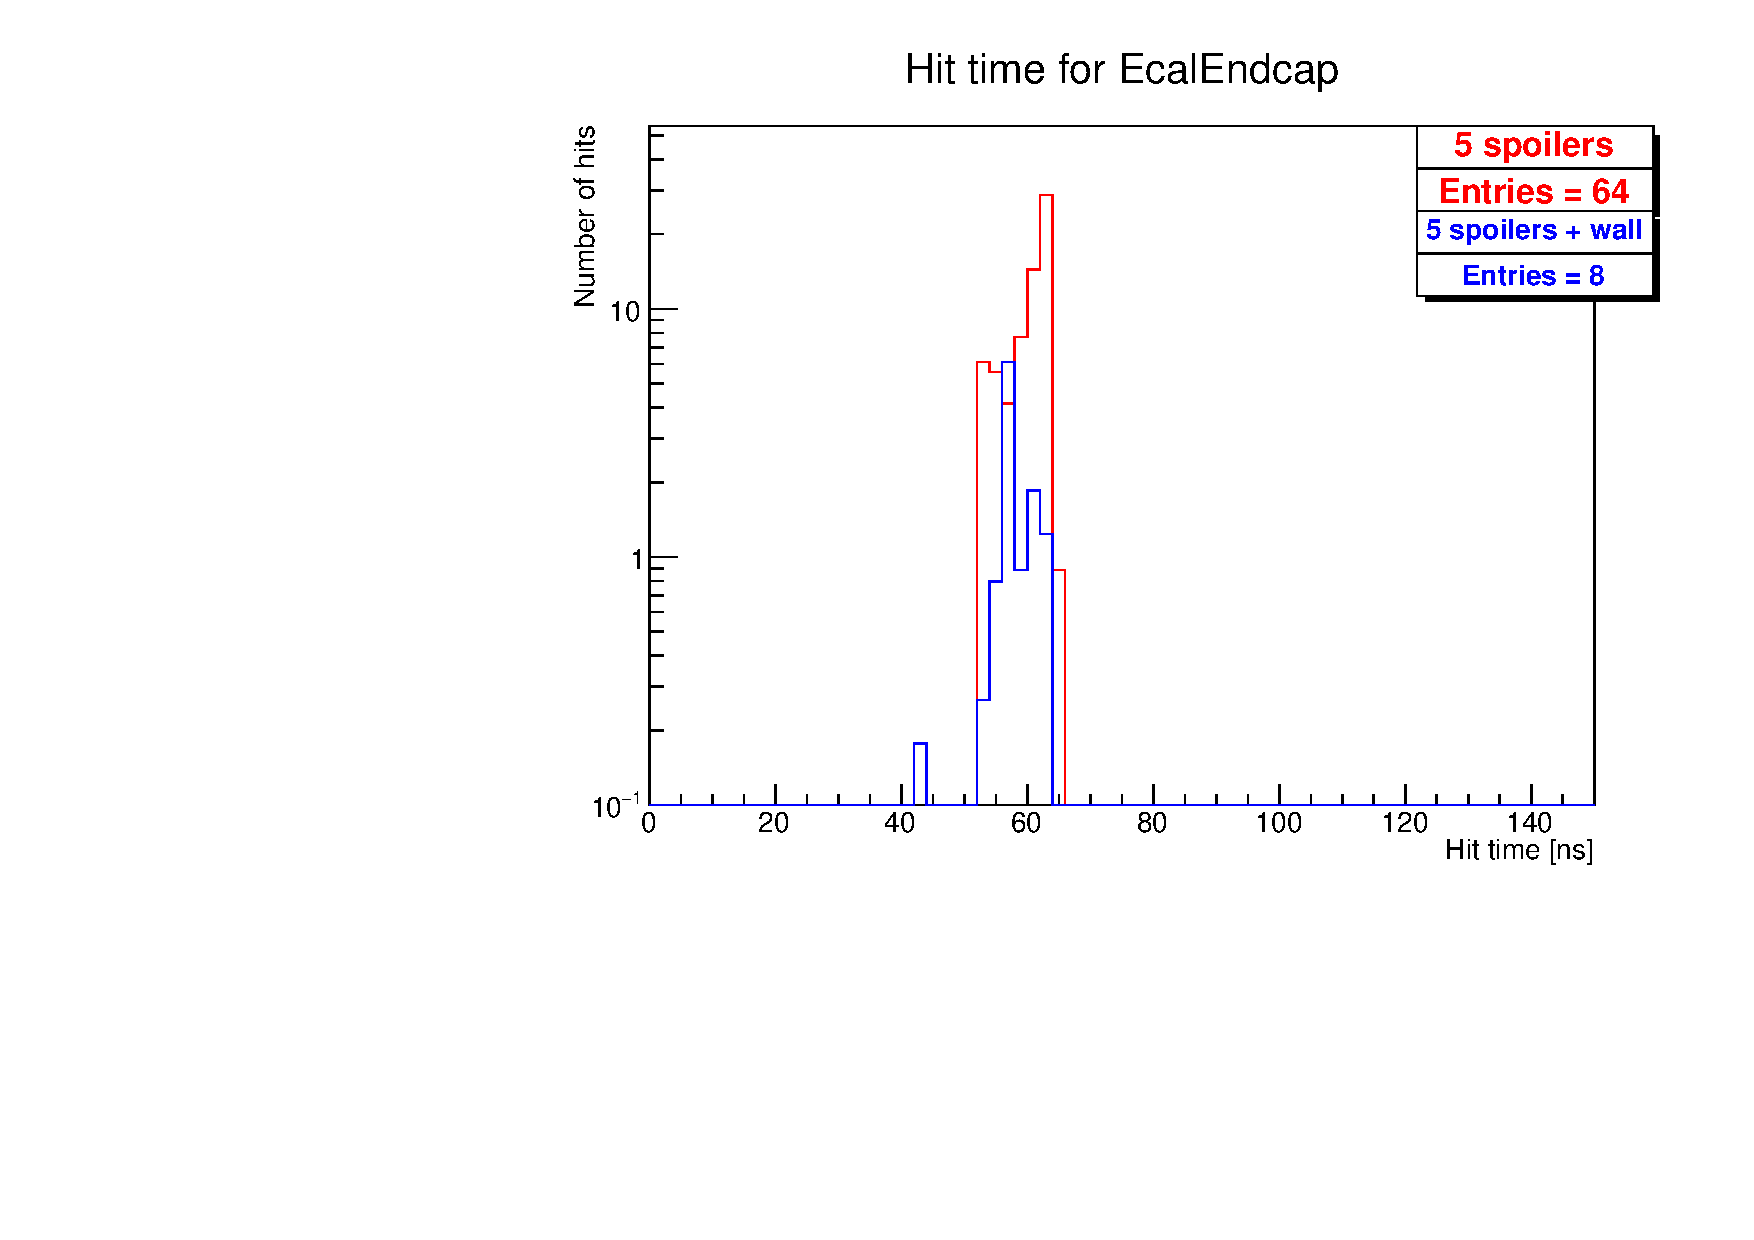
\includegraphics[height=0.26\textheight]{figures/muon_hittime_all_layers_shower_EcalEndcap.pdf}
        \caption{Hit time of the shower particles}
        \label{fig:hittime_shower_ECAL}
    \end{subfigure}
    \caption[Hit time distributions in the ECAL endcaps]{
    The distributions of the hit time of the primary muons and the shower particles hitting the ECAL endcaps.
    For both shielding scenarios, the time distributions are similar.
    The primary muons leave hits between about 23 and \unit{50}{ns} after the bunch crossing, since they have to travel through the whole detector before they reach the ECAL endcaps.
    The shower particles on the other hand hit the ECAL endcaps about \unit{60}{ns} after the crossing.
    }
    \label{fig:Hit_time}
\end{figure}